\chapter{L'incident du peuplier}
\keywords{Contemporain}{Action}{Militaire, diplomatie, guerre froide}

\section{Scénario}

Ce scénario est inspiré d'un fait réel ayant eu lieu en août 1976 (le \emph{poplar tree incident})\footnote{\url{https://fr.wikipedia.org/wiki/Incident_du_peuplier}} dans la zone démilitarisée (DMZ) séparant la Corée du Nord de la Corée du Sud.
Comme beaucoup d'autres incidents diplomatiques de l'époque, la tension découle en grande partie du contexte de guerre froide entre deux superpuissances.

\subsection{Accroche}

Août 1976. Zone démilitarisée coréenne, section contrôlée par l'ONU. Un groupe de soldats coréens et américains s'apprête à tailler les branches d'un peuplier car celles-ci masquent leur ligne de vue sur le \og pont de Non-retour\fg.
Ledit pont est l'unique passage permettant aux nord-coréens de traverser la rivière Sachon pour rejoindre leur propre zone.
Quinze minutes plus tard, un camion de soldats nords-coréens arrive.
Ils demandent aux onusiens de stopper l'élagage de l'arbre car celui-ci aurait été planté par Kim Il-sung en personne.
Devant leur refus, ils attaquent le contingent à coups de hachettes et de gourdins, tuant deux officiers américains et capturant plusieurs soldats.

\subsection{Péripéties}

L'incident enflamme la zone.
Les nord-coréens dénoncent une agression américaine et reçoivent le soutien immédiat de Cuba et de nombreux pays non-alignés.
En face, la CIA considère que l'attaque nord-coréenne était préméditée et les États-Unis passent en DEFCON3.

Les commandement de l'ONU ou l'état-major des États-Unis mobilise les personnages dans le cadre de l'opération \emph{Paul Bunyan}, du nom de légendaire bûcheron américain.

Des sapeurs du corps d'ingiénerie de l'armée de terre sont diligentés pour abattre l'arbre.
Un bataillon de soldats américains est envoyé comme escorte, épaulé par les forces spéciales coréennes.
En appui de cette démonstration de force, plusieurs hélicoptères et avions de combat sont déployés dans l'espoir d'intimider le régime nord-coréen.
Les forces armées pénètrent ainsi dans la DMZ et l'impressionnante armada converge vers le peuplier à deux pas du pont de non-retour.
Très rapidement, plusieurs bus militaires nord-coréens arrivent sur site pour préparer la riposte.
Des soldats en descendent et déploient des mitrailleuses sur l'autre rive.

L'objectif de l'opération \emph{Paul Bunyan} est simple: abattre le peuplier tout en évitant la guerre.

Le tableau de la page \pageref{table:peuplier} comporte quelques événements aléatoires permettant d'épicer la situation et de maintenir les joueuses sur le qui-vive.

\subsection{Résolution}

En fonction des décisions du groupe et de leurs réactions aux événements, le conflit peut très facilement être désamorcé (après tout, l'équilibre des forces est très en défaveur des nords-coréens).
Même une escarmouche ou une fusillade, si elle est maintenue sous contrôle, ne risque pas de dégénérer en une guerre ouverte.
Cependant, la violence peut vite prendre de l'ampleur si personne ne s'en préoccupe.
L'idée est de mettre de scène une escalade lente mais inéluctable de l'opposition entre les deux factions et de jouer sur la tension qui l'accompagne.
Il ne faut donc pas hésiter à rendre les choses difficiles pour les personnages: rien ne doit se passer comme prévu et chaque petite erreur ou entorse aux consignes a le potentiel d'être l'étincelle qui met le feu aux poudres.

\begin{table}
	\caption{Événements aléatoires durant l'abattage du peuplier}
	\label{table:peuplier}
	\colortablerows
	\begin{tabularx}{0.9\textwidth}{cX}
	d8 & Événement\\
	1  & Les tronçonneuses tombent en panne après quelques minutes. Il faut soit en faire venir des nouvelles, soit finir le travail à la hache.\\
	2  & Un soldat américain s'avance sur le pont et provoque les nord-coréens. Il se trouve qu'il est proche d'un des officiers assassinés.\\
	3  & Des camions nord-coréens s'installent à 150m\dots et construisent un nouveau pont.\\
	4  & Les nord-coréens font s'avancer les prisonniers sur le pont. Ils seront relâchés si les forces impérialistes renoncent, sinon ils seront exécutés.\\
	5  & Un des soldats sud-coréens se comporte étrangement. Il transmet discrètement des informations au régime du nord sur l'avancée de l'opération américaine.\\
	6  & Les renseignements japonais ont intercepté un message nord-coréens : leurs troupes s'apprêteraient à bloquer la rivière Imjin. C'est malheureusement la route prévue par le commandement de l'ONU pour une évacuation par canots en cas d'attaque\dots\\
	7  & Un jeune nord-coréen saute dans la rivière et tente de traverser à la nage. Il appelle à l'aide en anglais et jure qu'il veut faire défection.\\
	8  & Alors que les sapeurs ramassent les branches déjà coupées et les chargent dans un pick-up conformément aux ordres, les sud-coréens leur demandent de les laisser sur place. Compte-tenu du symbolisme de l'arbre, les nords-coréens pourraient prendre cet acte pour une provocation.\\
	\end{tabularx}
\end{table}

\subsection*{Lieu: la zone jointe de sécurité}

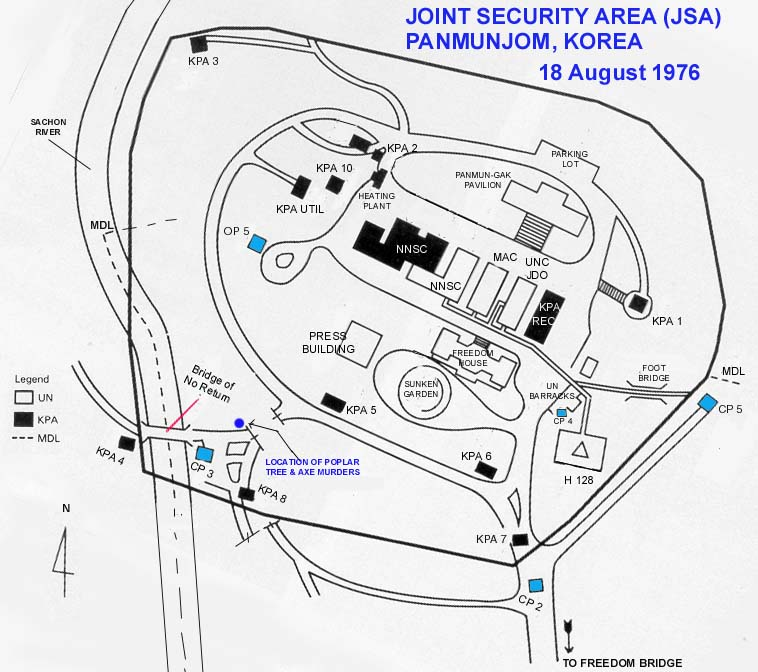
\includegraphics[width=\textwidth]{images/Joint_Security_Area_1976_map.jpg}

\illustration{chainsaw}
